\documentclass[a4paper,12pt]{article}
\usepackage{geometry}
\usepackage[utf8]{inputenc}
\usepackage{amssymb}
\usepackage[greek,english]{babel}
\usepackage{amsmath}
\usepackage[scheme=plain]{ctex}
\usepackage{multirow}
\usepackage{multicol}
\usepackage{mathrsfs}
\usepackage{enumerate}
\usepackage{algorithm}
\usepackage{algpseudocode}
\usepackage{graphicx} 
\geometry{left=2.0cm,right=2.0cm,top=2.0cm,bottom=2.0cm}
\usepackage{CJK}
\usepackage{float}
\usepackage{tabularx}
\usepackage{makecell}
\usepackage{mathabx}
\usepackage{tikz}
\usepackage{pgf}
\usepackage{caption}
\usepackage{subcaption}
\usepackage{listings}
\usepackage{xcolor}
\usepackage[colorlinks,linkcolor=black]{hyperref}
\usepackage{breakurl}
\usepackage{textcomp}
\usepackage{bm}
\usepackage{booktabs}
\usepackage{fancyhdr}
\usepackage{hyperref}
\usepackage{url}
\usepackage{verbatim}
\def\UrlBreaks{\do\A\do\B\do\C\do\D\do\E\do\F\do\G\do\H\do\I\do\J
\do\K\do\L\do\M\do\N\do\O\do\P\do\Q\do\R\do\S\do\T\do\U\do\V
\do\W\do\X\do\Y\do\Z\do\[\do\\\do\]\do\^\do\_\do\`\do\a\do\b
\do\c\do\d\do\e\do\f\do\g\do\h\do\i\do\j\do\k\do\l\do\m\do\n
\do\o\do\p\do\q\do\r\do\s\do\t\do\u\do\v\do\w\do\x\do\y\do\z
\do\.\do\@\do\\\do\/\do\!\do\_\do\|\do\;\do\>\do\]\do\)\do\,
\do\?\do\'\do+\do\=\do\#}


\begin{document}
	\begin{center}
		{
		\Large
		\textbf{ECE650 Malloc Library Part 1}\\
		\normalsize
		}
	\end{center}
	
	\section{Requirements \& Summary of Developments}
	\subsection{Project requirements}
	\subsubsection{\texttt{malloc} and \texttt{free} functions}
	\par The template of \texttt{malloc} function is: $\texttt{void * malloc (size\_t size);}$
	\par \texttt{malloc} takes a parameter of type \texttt{size\_t}, which indicates the number of bytes users need. It returns a pointer of type \texttt{void *} that points to the allocated memory. 
	\par When the \texttt{malloc} function is called, it returns the address of an allocated block. On failure, it returns \texttt{NULL}. 
	\par The template of \texttt{free} function is: $\texttt{void free (void * ptr);}$
	\par \texttt{free} takes a parameter of type \texttt{void *}, which indicates the memory address that needs to be released. 
	\par When the \texttt{free} function is called, it checks whether the pointer is within the heap. If not, return directly. If so, mark the block as free and release it back to the memory. 
	\subsubsection{Environment \& tools}
	\par We developed the \texttt{malloc} library in C language under Linux system. Using the \texttt{Makefile} provided, we built the source files into a library that can be called outside the current directory. 
	\subsection{Report organization}
	\par In \textbf{Section 2}, we discussed the design and implementation, including data structures and algorithms; testing is also discussed here. In \textbf{Section 3}, we discussed the results and performance analyses, including operation time and fragmentation. \textbf{Section 4} is the reference. 
	\section{Design, Implementation \& Testing}
	\subsection{Design choices}
	\par In this project, we used extra memory space to store the block information. 
	\begin{figure}[H]
		\centering
		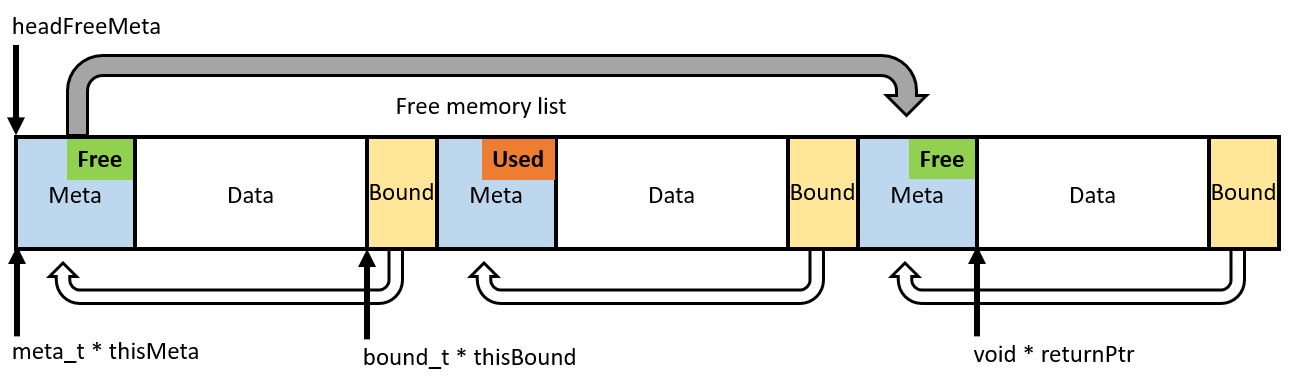
\includegraphics[width=1.1\linewidth]{1.png}
	\end{figure}
	\subsubsection{Memory block structure}
	\par The memory block consists of three parts: metadata, data space and bound. 
	\par The metadata (of type \texttt{meta\_t}) stores the size of the data space (which is always aligned to a multiple of 16), a flag to indicate the free status and a pointer to the metadata of the next free memory block (\texttt{NULL} if the block itself is not in the free list). 
	\par The bound contains 1 field: \texttt{thisMeta}, which is a pointer (of type \texttt{meta\_t}) to the metadata of the current block. It helps us to locate the current block from backward. 
	\par When \texttt{malloc} allocates a block, the address of the data space is returned to the user. 
	\subsubsection{Free list structure}
	\par A free list is designed to store the address of free memory blocks. 
	\par The free list is a linked list. In \texttt{my\_malloc.h}, a static variable \texttt{headFreeMeta} is defined. It indicates the head of the free list. Every pointer in the list is of type \texttt{meta\_t}, pointing to the meta address of the next free block. The addresses in the list are in ascending order. 
	\subsection{Implementation logic}
	\subsubsection{Fit block searching}
	\par Two policies are supported in this project: first-fit and best-fit. In both policies, \texttt{malloc} traverses the free list and checks the size of each block. On first-fit, once \texttt{malloc} finds a block of enough space, it makes use of the block without further checking. On best-fit, \texttt{malloc} examines all free blocks and uses the one with enough but smallest space. It stops traversing in advance only if it founds a block which has just enough space. 
	\par Both \texttt{ff\_malloc} and \texttt{bf\_malloc} calls the function \texttt{perform\_malloc} with template $$\texttt{void * perform\_malloc(size\_t inSize, void * (* get\_fit)(size\_t));}$$ 
	It will calls either \texttt{get\_ff\_fit} or \texttt{get\_bf\_fit} to search for free blocks. 
	\subsubsection{Function logic}
	\par \textbf{\textbf{\texttt{malloc}} working flow}
	\par When either \texttt{ff\_malloc} or \texttt{bf\_malloc} is called, it will call the function \texttt{perform\_malloc}. \texttt{perform\_malloc} will then use the function pointer (which points to either \texttt{get\_ff\_fit} or \texttt{get\_bf\_fit}) to get the suitable memory block. Both \texttt{get\_ff\_fit} and \texttt{get\_bf\_fit} check the size of the block: if there is enough space for a new block, it will split the current block (function \texttt{split\_block}) into two parts and return the pointer of the latter one; otherwise, it simply returns the found block and remove the pointer from the free list (function \texttt{delete\_node}). 
	\par \texttt{malloc} uses the function \texttt{renew\_info\_malloc} to mark the block as allocated and then return the pointer to the data space. \\
	\textbf{\textbf{\texttt{free}} working flow}
	\par When either \texttt{ff\_free} or \texttt{bf\_free} is called, it will call the function \texttt{perform\_free}. \texttt{perform\_free} will use the get to the meta part of the block and mark it as free and try to merge the block with other blocks (function \texttt{merge\_back} and \texttt{merge\_front}). 
	\par \texttt{merge\_back} checks whether the next block is free. If so, it deletes the next block from free list (function \texttt{delete\_node}) and changes the settings of the newly created block. \texttt{merge\_front} is used after \texttt{merge\_back}, which checks whether the previous block is free. If so, it changes the settings of blocks; if not, it adds the current block to the free list (function \texttt{add\_node}). 
	\subsection{Testing}
	\par The code was tested on the ECE551 VM with both the provided kit and some other cases. 
	\par When developing, I used \texttt{general\_tests} to check whether the pointer arithmetic was done correctly. After that, I used the \texttt{alloc\_policy\_tests} to check whether the codes worked efficiently. At first, \texttt{malloc} worked unusually fast, so I added extra codes to print messages about how functions allocated space, freed pointers, merged and split blocks. By checking the printed free list, I noticed that the list was not successfully built, so I fixed the code. After debugging, I wrote an extra test file to allocate space for different types of variables (\texttt{int}, \texttt{char}, \texttt{char*}, etc.). The cases are designed to get different results for FF and BF. By comparing the printed messageand hand-calculated results, I double-checked that the codes could work. 
	
	\section{Performance Results \& Analysis}
	\par Our \texttt{malloc} and \texttt{free} got stable results on intensive tests. For equal size, we ran 3 same tests and got the average; for small and large allocation, we set the random seed to 0, 1 and 2 and got averages after 3 tests respectively. The results are as follows:
\begin{table}[H]
  \centering
    \begin{tabular}{c|c|c|c|c}
          & \multicolumn{2}{c|}{FF} & \multicolumn{2}{c}{BF} \\
    \hline
          & \multicolumn{1}{l|}{Time} & \multicolumn{1}{l|}{Fragmentation} & \multicolumn{1}{l|}{Time} & \multicolumn{1}{l}{Fragmentation} \\
    \hline
    Equal & 20.14838 & 0.999889 & 20.16704 & 0.999889 \\
    \hline
    Small & 9.215181 & 0.624184 & 2.623498 & 0.904712 \\
    \hline
    Large & 51.66187 & 0.843796 & 61.26451 & 0.960573 
    \end{tabular}
\end{table}
	\par Both policies got almost the same results for equal-size, because both returns the first free block. For small-range allocation, FF works slower than BF and gets a lower fragmentation. For large-range allocation, FF works faster than BF and gets a lower fragmentation. Both fragmentations rise when range goes larger, because the rising range raises the uncertainties of block sizes and creates more split blocks. 
	\par In both situations, BF got a higher fragmentation because it always chooses the block with smallest allowable size. When blocks are just a little larger than requested, they will be split into two part: one block for user and another block that has such a small size that it is nearly impossible to be reused. A possible explanation for BF'S faster run time on small-range is that BF traverses through the list and is less likely to need splitting and merging; but when range becomes larger, FF overtakes BF because it needs less time for list traversal. 
	\par Which policy to choose depends on user requirements. When users care more about time than fragmentation and only need small-range allocation at most time, they may choose BF. However, if users either want a higher efficiency on memory management or need to do many large-range allocations, FF is a better choice. 
	
	\section{References}
	\begin{itemize}
		\item[${[1]}$] Malloc. \textit{CS241: System Programming Coursebook}. University of Illinois. 
		\item[${[2]}$] Saelee, Michael. Mallow Slides. Illinois Institute of Technology. 
	\end{itemize}
	
	\begin{comment}
	\begin{figure}[H]
		\centering
		\includegraphics[width=0.4\linewidth]{Q2.png}
	\end{figure}
	\end{comment}
	

\end{document}
